\appendix
\addcontentsline{toc}{section}{Appendice}

\section{Resoconto attività di verifica}
	
\subsection{Verifica processi}

\subsubsection{Calcolo metriche gestione delle risorse - QP1}
Per verificare che i costi stabiliti rientrino in quanto preventivato si trovano a seguire dei grafici contenenti i risultati ottenuti:

	\paragraph{Budgeted cost of work scheduled}
		\begin{figure}[H]
			\centering
			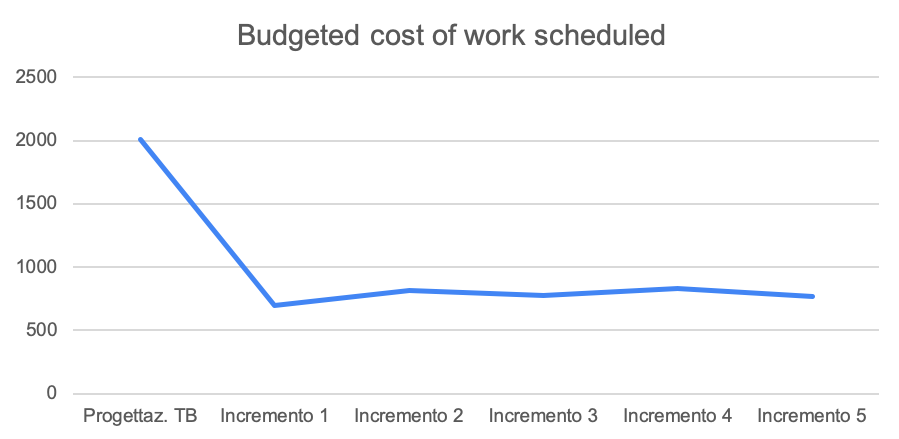
\includegraphics[width=0.8\linewidth]{./res/images/BCWS_1.png}
			\caption{Grafico contenente il costo preventivato in euro per fase}
			\label{fig:Grafico contenente il costo preventivato in euro per fase}
		\end{figure}
		\begin{figure}[H]
			\centering
			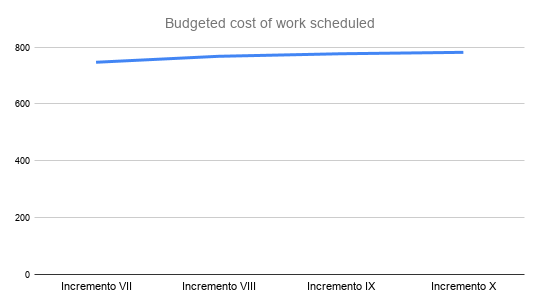
\includegraphics[width=0.8\linewidth]{./res/images/BCWS_2.png}
			\caption{Grafico contenente il costo preventivato in euro per fase}
			\label{fig:Grafico contenente il costo preventivato in euro per fase}
		\end{figure}

	\paragraph{Actual cost of work performed}
		\begin{figure}[H]
			\centering
			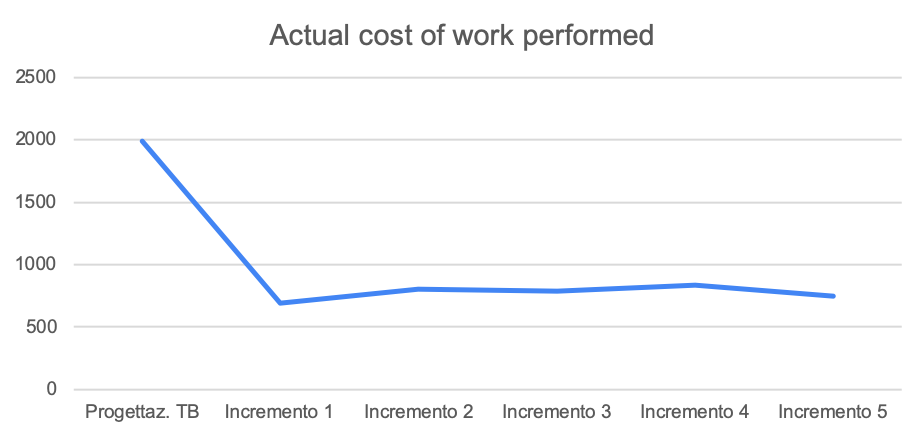
\includegraphics[width=0.8\linewidth]{./res/images/ACWP_1.png}
			\caption{Grafico contenente il costo effettivo in euro per fase}
			\label{fig:Grafico contenente il costo effettivo in euro per fase}
		\end{figure}
		\begin{figure}[H]
			\centering
			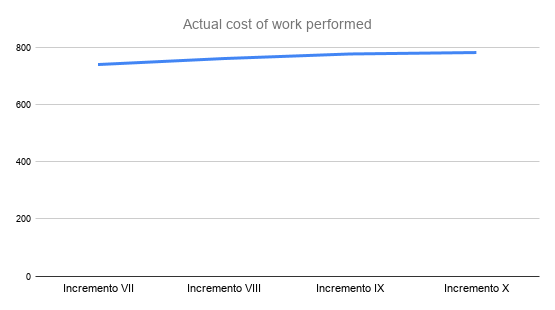
\includegraphics[width=0.8\linewidth]{./res/images/ACWP_2.png}
			\caption{Grafico contenente il costo effettivo in euro per fase}
			\label{fig:Grafico contenente il costo effettivo in euro per fase}
		\end{figure}

	\paragraph{Budgeted cost of work performed}
		\begin{figure}[H]
			\centering
			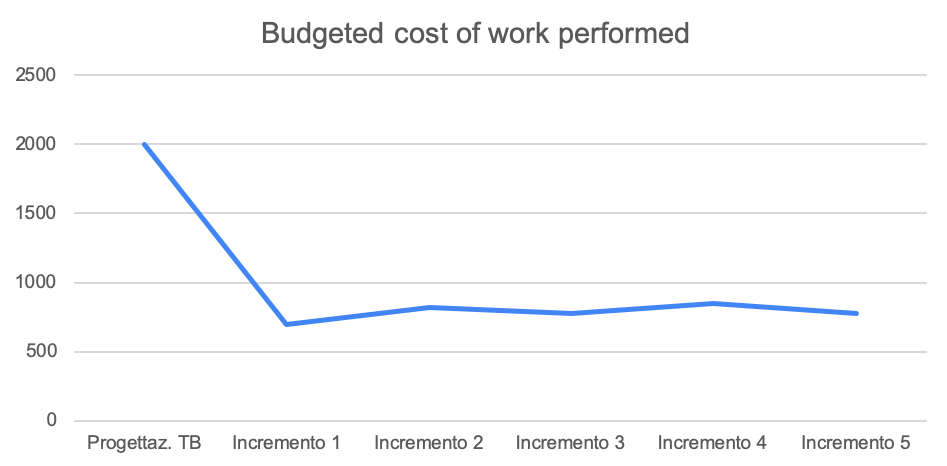
\includegraphics[width=0.8\linewidth]{./res/images/BCWP_1.png}
			\caption{Grafico contenente il valore del prodotto in euro per fase}
			\label{fig:Grafico contenente il valore del prodotto in euro per fase}
		\end{figure}
		\begin{figure}[H]
			\centering
			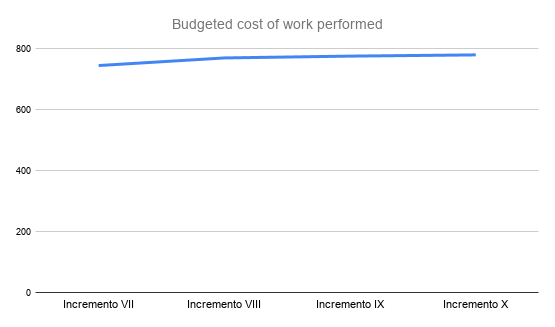
\includegraphics[width=0.8\linewidth]{./res/images/BCWP_2.png}
			\caption{Grafico contenente il valore del prodotto in euro per fase}
			\label{fig:Grafico contenente il valore del prodotto in euro per fase}
		\end{figure}

	\paragraph{Schedule variance}
		\begin{figure}[H]
			\centering
			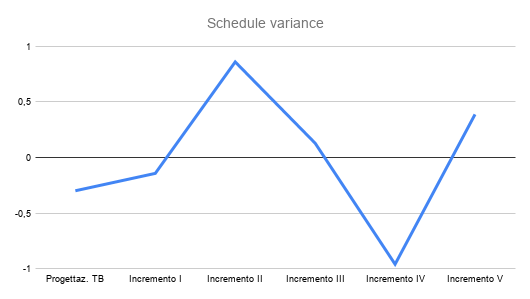
\includegraphics[width=0.8\linewidth]{./res/images/SV_1.png}
			\caption{Grafico contenente il valore dello schedule variance per fase}
			\label{fig:Grafico contenente il valore dello schedule variance per fase}
		\end{figure}
		\begin{figure}[H]
			\centering
			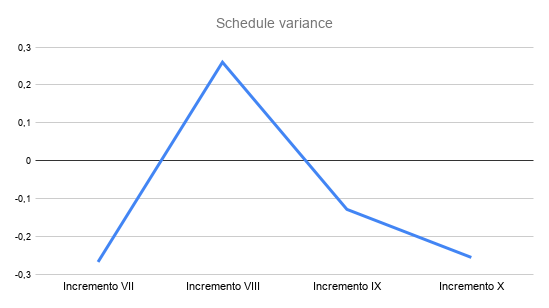
\includegraphics[width=0.8\linewidth]{./res/images/SV_2.png}
			\caption{Grafico contenente il valore dello schedule variance per fase}
			\label{fig:Grafico contenente il valore dello schedule variance per fase}
		\end{figure}


	\paragraph{Cost Variance}
		\begin{figure}[H]
			\centering
			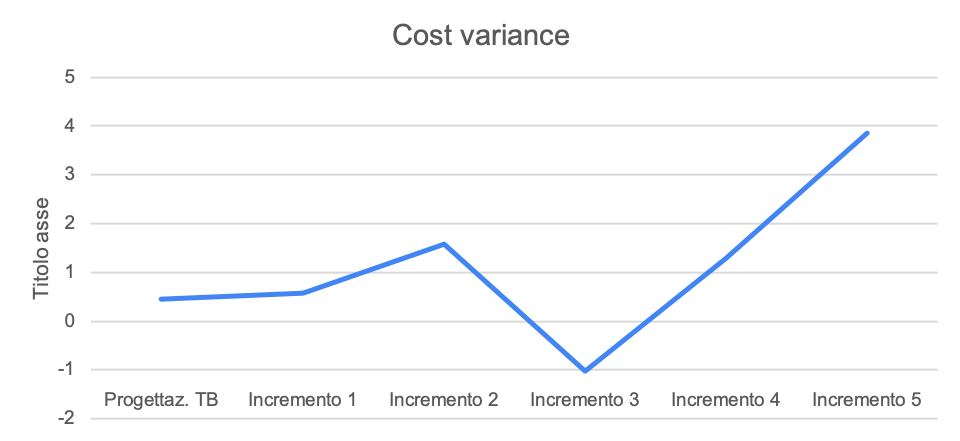
\includegraphics[width=0.8\linewidth]{./res/images/CV_1.png}
			\caption{Grafico contenente il valore dello cost variance per fase}
			\label{fig:Grafico contenente il valore dello cost variance per fase}
		\end{figure}
		\begin{figure}[H]
			\centering
			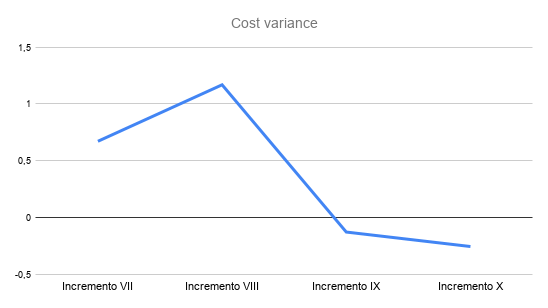
\includegraphics[width=0.8\linewidth]{./res/images/CV_2.png}
			\caption{Grafico contenente il valore dello cost variance per fase}
			\label{fig:Grafico contenente il valore dello cost variance per fase}
		\end{figure}

\subsubsection{Calcolo metriche gestione dei rischi - QP2}

\paragraph{Unbudgeted Risks}
Per monitorare i rischi non preventivati riscontrati durante l'avanzamento del progetto si sono raccolte le misurazioni nei seguenti grafici:

	\begin{figure}[H]
		\centering
		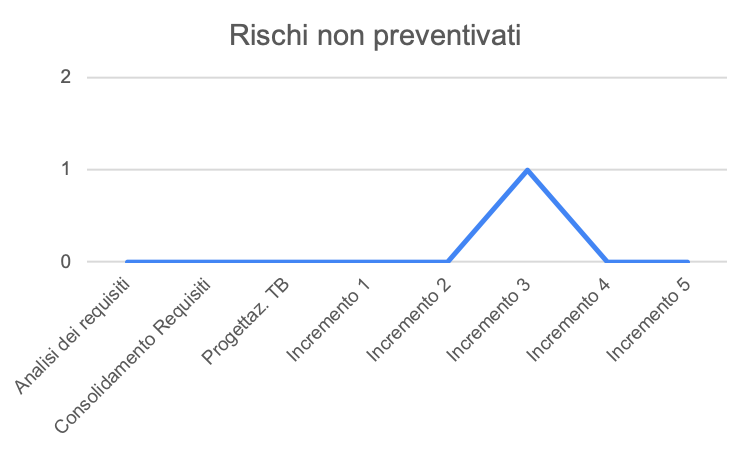
\includegraphics[width=0.8\linewidth]{./res/images/RischiNonPrevent_1.png}
		\caption{Grafico periodo/rischio della fase di analisi dei requisiti}
		\label{fig:Grafico periodo/rischio nel periodo di analisi dei requisiti}
	\end{figure}

	\begin{figure}[H]
			\centering
			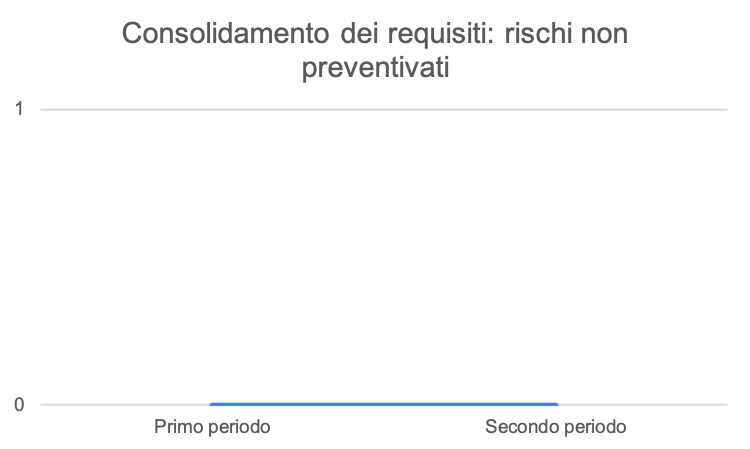
\includegraphics[width=0.8\linewidth]{./res/images/RischiNonPrevent_2.png}
			\caption{Grafico periodo/rischio per la fase di consolidamento dei requisiti}
			\label{fig:Grafico periodo/rischio per la fase di consolidamento dei requisiti}
	\end{figure}

	\begin{figure}[H]
			\centering
			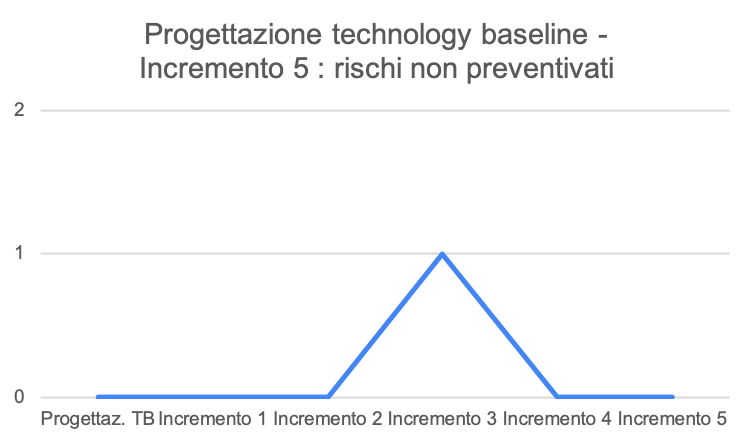
\includegraphics[width=0.8\linewidth]{./res/images/RischiNonPrevent_3.png}
			\caption{Grafico periodo/rischio per le fasi che vanno dalla progettazione della technology baseline all'incremento VI}
			\label{fig:Grafico periodo/rischio per le fasi che vanno dalla progettazione della technology baseline all'incremento VI}
	\end{figure}

	\begin{figure}[H]
			\centering
			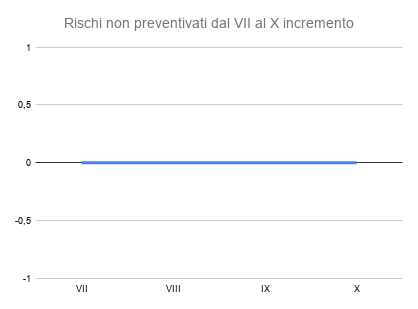
\includegraphics[width=0.8\linewidth]{./res/images/RischiNonPreven_4.png}
			\caption{Grafico periodo/rischio per le fasi che vanno dall'incremento VII all'incremento X}
			\label{fig:Grafico periodo/rischio per le fasi che vanno dall'incremento VII all'incremento X}
	\end{figure}

\subsubsection{Calcolo metriche sviluppo - QP3}
\paragraph{Satisfied mandatory requirements}
	\begin{figure}[H]
			\centering
			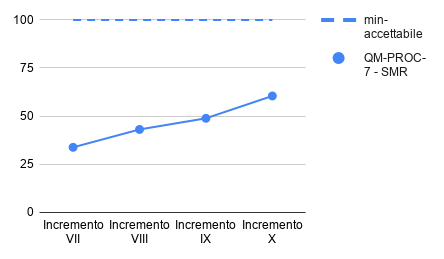
\includegraphics[width=0.8\linewidth]{./res/images/QM-PROC-7-SMR.png}
			\caption{Grafico periodo/percentuale di requisiti obbligatori soddisfatti per le fasi che vanno dall'incremento VII all'incremento X}
			\label{fig:Grafico periodo/percentuale di requisiti obbligatori soddisfatti per le fasi che vanno dall'incremento VII all'incremento X}
	\end{figure}
\paragraph{Satisfied desirable requirements}
	\begin{figure}[H]
			\centering
			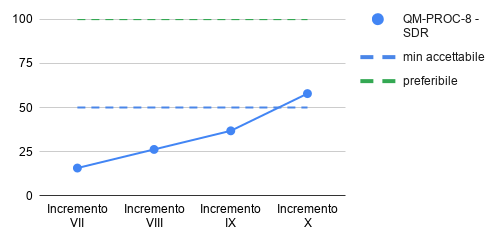
\includegraphics[width=0.8\linewidth]{./res/images/QM-PROC-8-SDR.png}
			\caption{Grafico periodo/percentuale di requisiti desiderabili soddisfatti per le fasi che vanno dall'incremento VII all'incremento X}
			\label{fig:Grafico periodo/percentuale di requisiti desiderabili soddisfatti per le fasi che vanno dall'incremento VII all'incremento X}
	\end{figure}
\paragraph{Satisfied optional requirements}
	\begin{figure}[H]
			\centering
			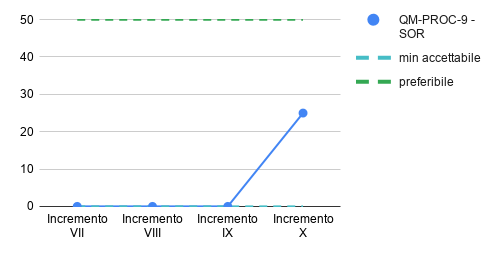
\includegraphics[width=0.8\linewidth]{./res/images/QM-PROC-9-SOR.png}
			\caption{Grafico periodo/percentuale di requisiti opzionali soddisfatti per le fasi che vanno dall'incremento VII all'incremento X}
			\label{fig:Grafico periodo/percentuale di requisiti opzionali soddisfatti per le fasi che vanno dall'incremento VII all'incremento X}
	\end{figure}
\paragraph{Numero di commit}
\begin{figure}[H]
			\centering
			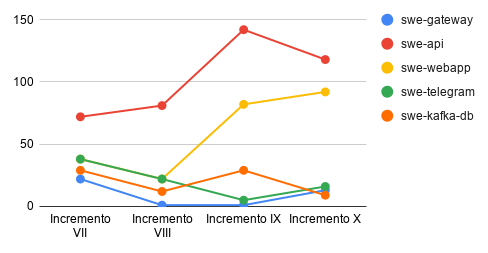
\includegraphics[width=0.8\linewidth]{./res/images/QM-PROC-10-NCOM.png}
			\caption{Grafico periodo/numero di commit per le fasi che vanno dall'incremento VII all'incremento X}
			\label{fig:Grafico periodo/numero di commit per le fasi che vanno dall'incremento VII all'incremento X}
	\end{figure}

\subsubsection{Calcolo metriche verifica - QP4}	
\paragraph{Code coverage}
\begin{figure}[H]
			\centering
			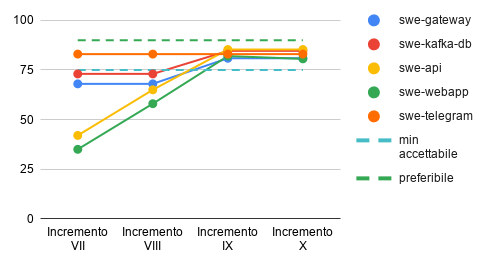
\includegraphics[width=0.8\linewidth]{./res/images/QM-TEST-1-COCO.png}
			\caption{Grafico periodo/percentuale di code coverage per le fasi che vanno dall'incremento VII all'incremento X}
			\label{fig:Grafico periodo/percentuale di code coverage per le fasi che vanno dall'incremento VII all'incremento X}
	\end{figure}
\paragraph{Condition coverage}
\begin{figure}[H]
			\centering
			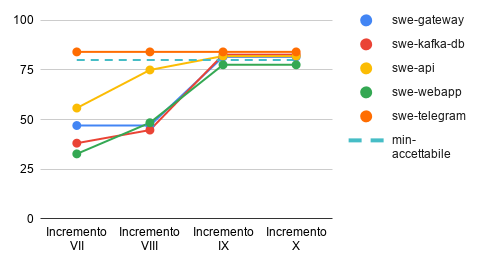
\includegraphics[width=0.8\linewidth]{./res/images/QM-TEST-2-CONCO.png}
			\caption{Grafico periodo/percentuale di condition coverage per le fasi che vanno dall'incremento VII all'incremento X}
			\label{fig:Grafico periodo/percentuale di condition coverage per le fasi che vanno dall'incremento VII all'incremento X}
	\end{figure}
\paragraph{Line coverage}
\begin{figure}[H]
			\centering
			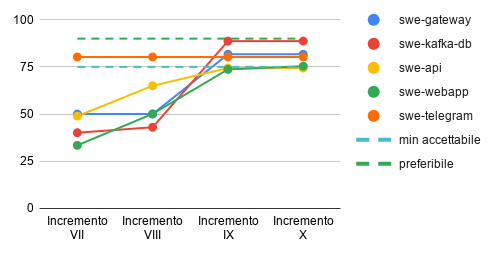
\includegraphics[width=0.8\linewidth]{./res/images/QM-TEST-3-LOCO.png}
			\caption{Grafico periodo/rischio per le fasi che vanno dall'incremento VII all'incremento X}
			\label{fig:Grafico periodo/rischio per le fasi che vanno dall'incremento VII all'incremento X}
	\end{figure}
\paragraph{Passed test cases percentage}
\begin{figure}[H]
			\centering
			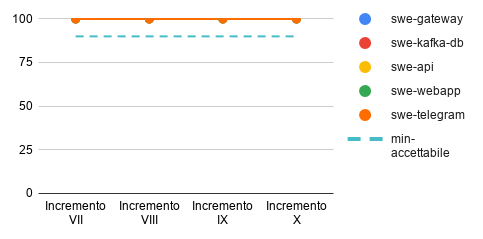
\includegraphics[width=0.8\linewidth]{./res/images/QM-TEST-4-PTCP.png}
			\caption{Grafico periodo/percentuale di test case passati per le fasi che vanno dall'incremento VII all'incremento X}
			\label{fig:Grafico periodo/percentuale di test case passati per le fasi che vanno dall'incremento VII all'incremento X}
	\end{figure}
\paragraph{Failed test cases percentage}
\begin{figure}[H]
			\centering
			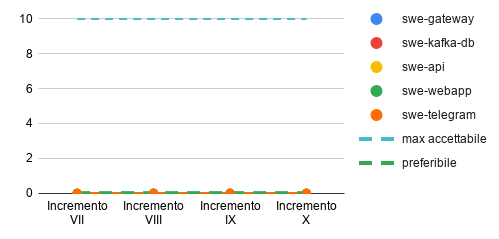
\includegraphics[width=0.8\linewidth]{./res/images/QM-TEST-5-FTCP.png}
			\caption{Grafico periodo/percentuale di test case falliti per le fasi che vanno dall'incremento VII all'incremento X}
			\label{fig:Grafico periodo/percentuale di test case falliti per le fasi che vanno dall'incremento VII all'incremento X}
	\end{figure}
\paragraph{Bug-fixing percentage}
\begin{figure}[H]
			\centering
			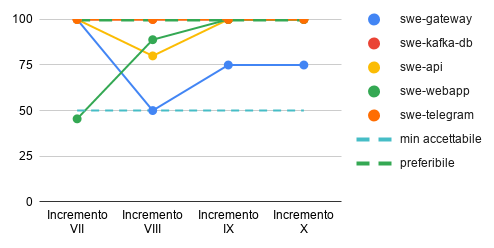
\includegraphics[width=0.8\linewidth]{./res/images/QM-TEST-6-BFP.png}
			\caption{Grafico periodo/percentuale di bug sistemati per le fasi che vanno dall'incremento VII all'incremento X}
			\label{fig:Grafico periodo/percentuale di bug sistemati per le fasi che vanno dall'incremento VII all'incremento X}
	\end{figure}
\paragraph{Complessità media dei test di classe}
\begin{figure}[H]
			\centering
			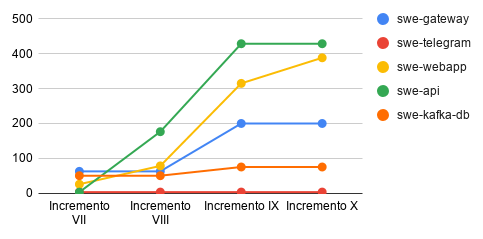
\includegraphics[width=0.8\linewidth]{./res/images/QM-TEST-7-CMTC.png}
			\caption{Grafico periodo/complessità media per le fasi che vanno dall'incremento VII all'incremento X}
			\label{fig:Grafico periodo/complessità media per le fasi che vanno dall'incremento VII all'incremento X}
	\end{figure}


\subsubsection{Calcolo metriche qualità - QP5}
\paragraph{Percentuale delle metriche soddisfatte}
\begin{figure}[H]
			\centering
			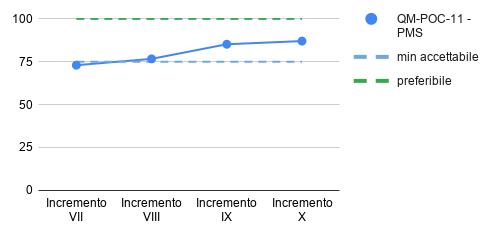
\includegraphics[width=0.8\linewidth]{./res/images/QM-PROC-11-PMS.png}
			\caption{Grafico periodo/percentuale metriche soddisfatte per le fasi che vanno dall'incremento VII all'incremento X}
			\label{fig:Grafico periodo/percentuale metriche soddisfatte per le fasi che vanno dall'incremento VII all'incremento X}
	\end{figure}

\subsection{Verifica prodotto}


\subsection{Verifica documentazione}

\subsubsection{Calcolo metriche comprensione - QC1}

\paragraph{Indice di Gulpease}
Per verificare quanto sono leggibili i documenti redatti si utilizza \glock{l'indice di Gulpease}, di seguito i grafici contenenti i risultati ottenuti:

\begin{figure}[H]
	\centering
	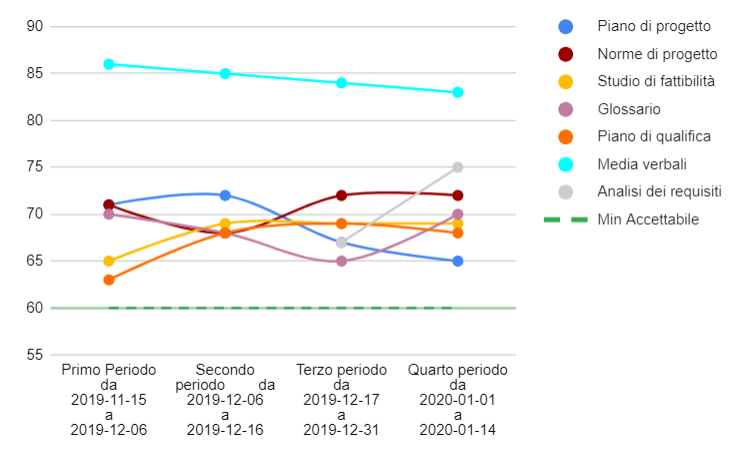
\includegraphics[width=0.8\linewidth]{./res/images/gulpease_1.png}
	\caption{Grafico periodo/indice di gulpease nel periodo di analisi dei requisiti.}
	\label{fig:Grafico indice di gulpease periodo di analisi dei requisiti.}
\end{figure}

\begin{figure}[H]
	\centering
	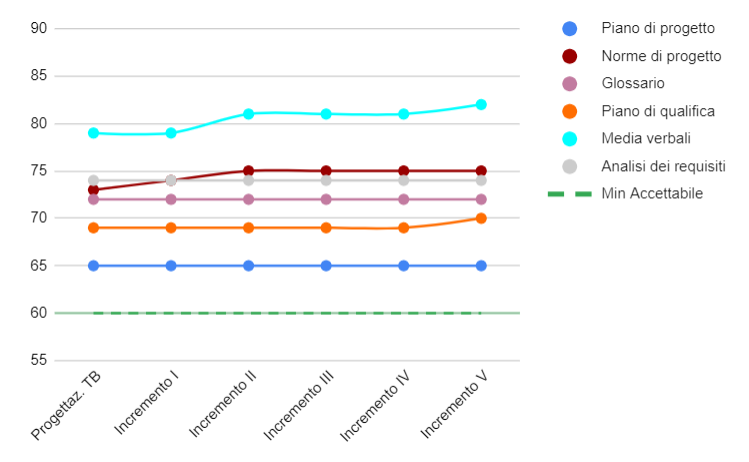
\includegraphics[width=0.8\linewidth]{./res/images/gulpease_2.png}
	\caption{Grafico periodo/indice di gulpease nel periodo di progettazione della technology baseline.}
	\label{fig:Grafico indice di gulpease periodo di progettazione della technology baseline.}
\end{figure}

\begin{figure}[H]
	\centering
	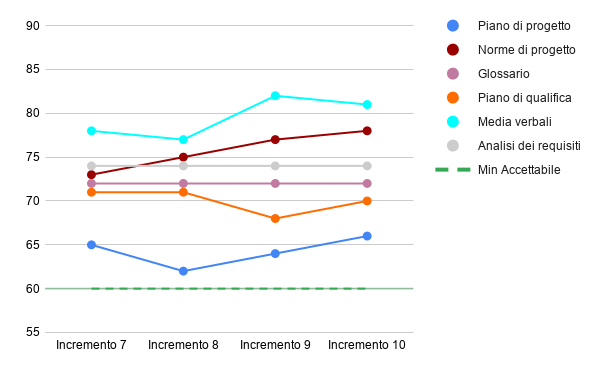
\includegraphics[width=0.8\linewidth]{./res/images/gulpease_3.png}
	\caption{Grafico periodo/indice di gulpease nel periodo dall'incremento VI al X.}
	\label{fig:Grafico indice di gulpease periodo dall'incremento VI al X.}
\end{figure}

\paragraph{Correttezza ortografica}
È stato effettuato un controllo di ortografia e di seguito vengono illustrati i grafici contenenti i risultati ottenuti:

\begin{figure}[H]
	\centering
	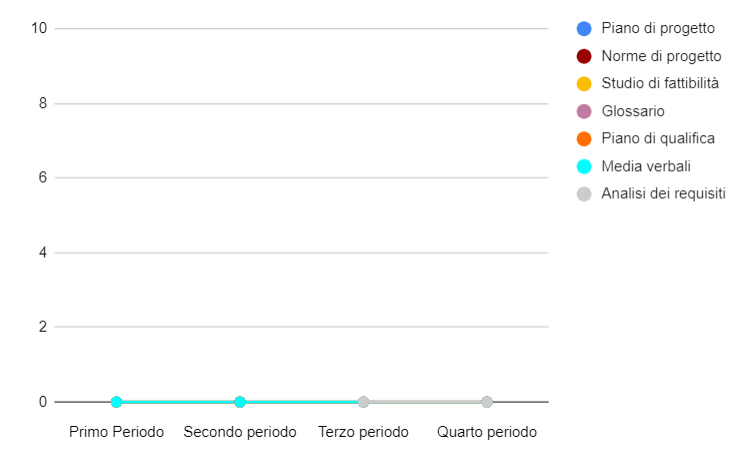
\includegraphics[width=0.8\linewidth]{./res/images/ortografia_1.png}
	\caption{Grafico periodo/errori ortografici nel periodo di analisi dei requisiti.}
	\label{fig:Grafico errori ortografici durante il periodo di analisi dei requisiti.}
\end{figure}

\begin{figure}[H]
	\centering
	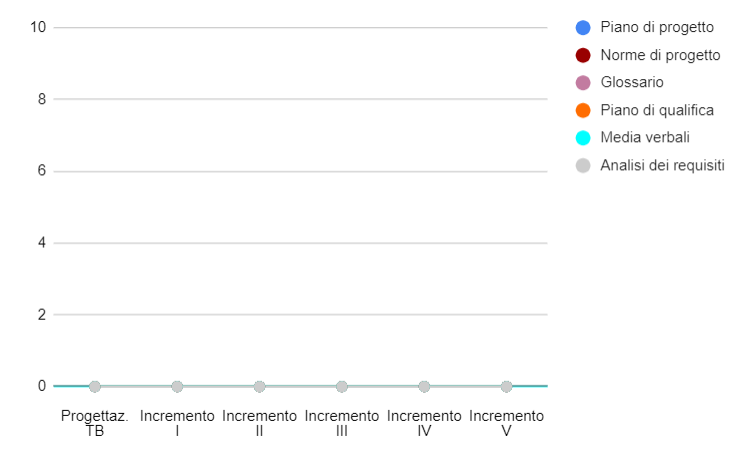
\includegraphics[width=0.8\linewidth]{./res/images/ortografia_2.png}
	\caption{Grafico periodo/errori ortografici nel periodo di progettazione della technology baseline.}
	\label{fig:Grafico errori ortografici durante il periodo di progettazione della technology baseline.}
\end{figure}

\begin{figure}[H]
	\centering
	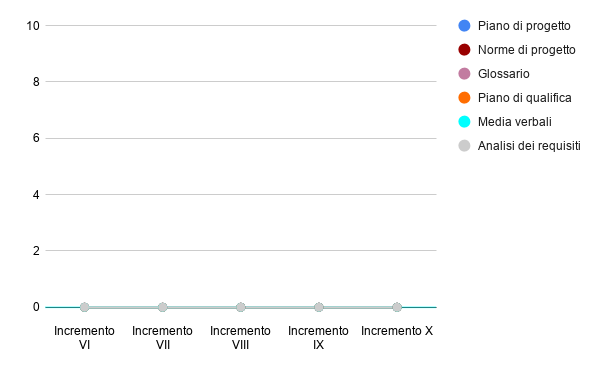
\includegraphics[width=0.8\linewidth]{./res/images/ortografia_3.png}
	\caption{Grafico periodo/errori ortografici nel periodo dall'incremento VI al X.}
	\label{fig:Grafico errori ortografici durante il periodo dall'incremento VI al X.}
\end{figure}

\paragraph{Limite lunghezza video tutorial}
\begin{figure}[H]
			\centering
			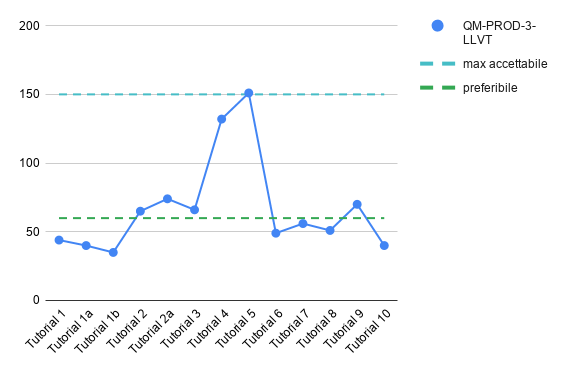
\includegraphics[width=0.8\linewidth]{./res/images/LLVT.png}
			\caption{Grafico periodo/lunghezza video per le fasi che vanno dall'incremento VII all'incremento X}
			\label{fig:Grafico periodo/lunghezza video per le fasi che vanno dall'incremento VII all'incremento X}
	\end{figure}

\subsubsection{Calcolo metriche sicurezza - QC2}
\paragraph{Numero di vulnerabilità rilevate}
\begin{figure}[H]
			\centering
			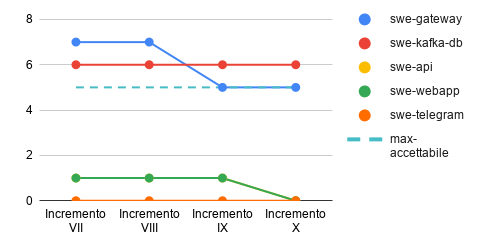
\includegraphics[width=0.8\linewidth]{./res/images/QM-PROD-4-NVUL.png}
			\caption{Grafico periodo/numero di vulnerabilità per le fasi che vanno dall'incremento VII all'incremento X}
			\label{fig:Grafico periodo/numero di vulnerabilità per le fasi che vanno dall'incremento VII all'incremento X}
	\end{figure}
\paragraph{Tempo di risoluzione vulnerabilità}
\begin{figure}[H]
			\centering
			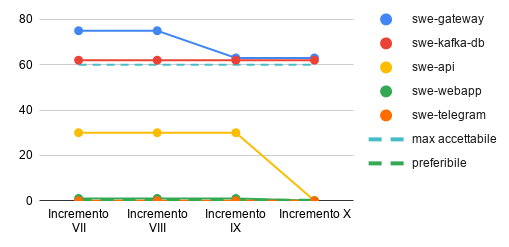
\includegraphics[width=0.8\linewidth]{./res/images/QM-PROD-5-TVUL.png}
			\caption{Grafico periodo/tempo di risoluzione per le fasi che vanno dall'incremento VII all'incremento X}
			\label{fig:Grafico periodo/tempo di risoluzione per le fasi che vanno dall'incremento VII all'incremento X}
	\end{figure}

\subsubsection{Calcolo metriche affidabilità - QC3}
\paragraph{Numero di bug rilevati}
\begin{figure}[H]
			\centering
			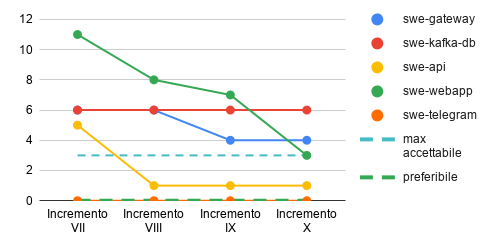
\includegraphics[width=0.8\linewidth]{./res/images/QM-PROD-6-NBUG.png}
			\caption{Grafico periodo/numero di bug per le fasi che vanno dall'incremento VII all'incremento X}
			\label{fig:Grafico periodo/numero di bug  per le fasi che vanno dall'incremento VII all'incremento X}
	\end{figure}
\paragraph{Tempo stimato risoluzione bug}
\begin{figure}[H]
			\centering
			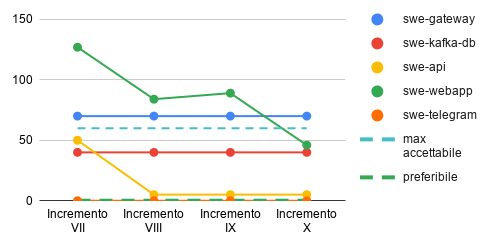
\includegraphics[width=0.8\linewidth]{./res/images/QM-PROD-7-TBUG.png}
			\caption{Grafico periodo/tempo di risoluzione per le fasi che vanno dall'incremento VII all'incremento X}
			\label{fig:Grafico periodo/tempo di risoluzione per le fasi che vanno dall'incremento VII all'incremento X}
	\end{figure}

\subsubsection{Calcolo metriche efficienza - QC4}
\paragraph{Risposta media}
\begin{figure}[H]
			\centering
			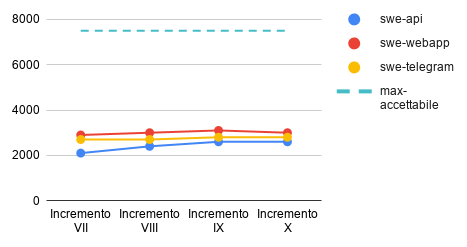
\includegraphics[width=0.8\linewidth]{./res/images/QM-PROD-8-RM.png}
			\caption{Grafico periodo/risposta media per le fasi che vanno dall'incremento VII all'incremento X}
			\label{fig:Grafico periodo/risposta media per le fasi che vanno dall'incremento VII all'incremento X}
	\end{figure}

\subsubsection{Calcolo metriche usabilità - QC5}
\paragraph{Profondità dell'albero delle azioni}
\begin{figure}[H]
			\centering
			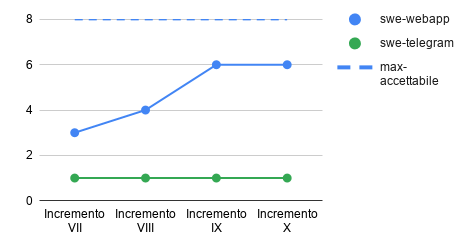
\includegraphics[width=0.8\linewidth]{./res/images/QM-PROD-9-PAA.png}
			\caption{Grafico periodo/numero di click per le fasi che vanno dall'incremento VII all'incremento X}
			\label{fig:Grafico periodo/numero di click per le fasi che vanno dall'incremento VII all'incremento X}
	\end{figure}
\paragraph{Profondità dell'albero delle pagine}
\begin{figure}[H]
			\centering
			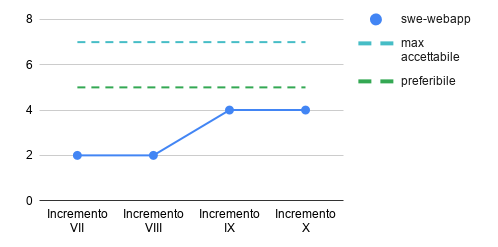
\includegraphics[width=0.8\linewidth]{./res/images/QM-PROD-10-PAP.png}
			\caption{Grafico periodo/profondità pagine per le fasi che vanno dall'incremento VII all'incremento X}
			\label{fig:Grafico periodo/profondità pagine per le fasi che vanno dall'incremento VII all'incremento X}
	\end{figure}

\subsubsection{Calcolo metriche manutenibilità - QC6}
\paragraph{Complessità ciclomatica media}
\begin{figure}[H]
			\centering
			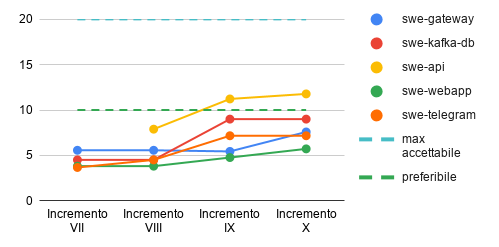
\includegraphics[width=0.8\linewidth]{./res/images/QM-PROD-11-COCIM.png}
			\caption{Grafico periodo/complessità ciclomatica per le fasi che vanno dall'incremento VII all'incremento X}
			\label{fig:Grafico periodo/complessità ciclomatica per le fasi che vanno dall'incremento VII all'incremento X}
	\end{figure}
\paragraph{Complessità della classe}
\begin{figure}[H]
			\centering
			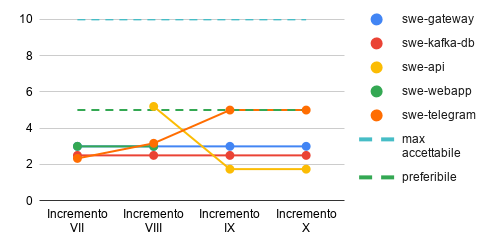
\includegraphics[width=0.8\linewidth]{./res/images/QM-PROD-12-CCLA.png}
			\caption{Grafico periodo/complessità per le fasi che vanno dall'incremento VII all'incremento X}
			\label{fig:Grafico periodo/complessità per le fasi che vanno dall'incremento VII all'incremento X}
	\end{figure}
\paragraph{Numero di code smell rilevati}
\begin{figure}[H]
			\centering
			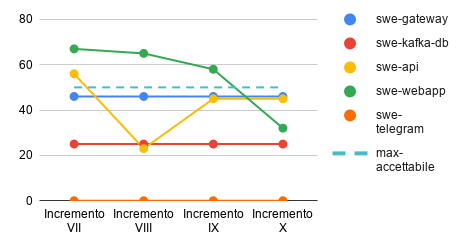
\includegraphics[width=0.8\linewidth]{./res/images/QM-PROD-13-NCS.png}
			\caption{Grafico periodo/numero di code smell per le fasi che vanno dall'incremento VII all'incremento X}
			\label{fig:Grafico periodo/rischio per le fasi che vanno dall'incremento VII all'incremento X}
	\end{figure}
\paragraph{Tempo di risoluzione code smell}
\begin{figure}[H]
			\centering
			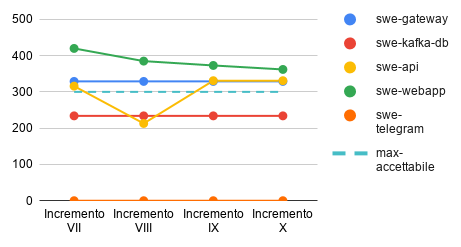
\includegraphics[width=0.8\linewidth]{./res/images/QM-PROD-14-TCS.png}
			\caption{Grafico periodo/tempo di risoluzione per le fasi che vanno dall'incremento VII all'incremento X}
			\label{fig:Grafico periodo/tempo di risoluzione per le fasi che vanno dall'incremento VII all'incremento X}
	\end{figure}
\paragraph{Percentuale di duplicazione del codice}
\begin{figure}[H]
			\centering
			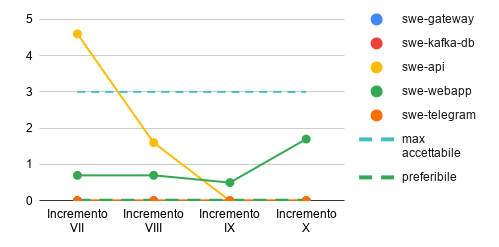
\includegraphics[width=0.8\linewidth]{./res/images/QM-PROD-15-DUPC.png}
			\caption{Grafico periodo/percentuale di duplicazione per le fasi che vanno dall'incremento VII all'incremento X}
			\label{fig:Grafico periodo/percentuale di duplicazione per le fasi che vanno dall'incremento VII all'incremento X}
	\end{figure}
\paragraph{Numero di violazioni standard di codifica}
\begin{figure}[H]
			\centering
			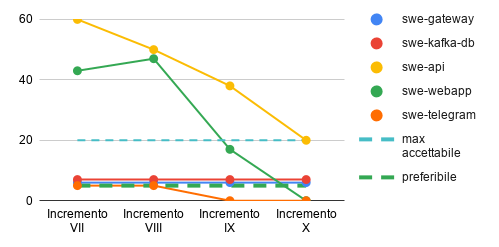
\includegraphics[width=0.8\linewidth]{./res/images/QM-PROD-16-NVSC.png}
			\caption{Grafico periodo/numero di violazione per le fasi che vanno dall'incremento VII all'incremento X}
			\label{fig:Grafico periodo/numero di violazione per le fasi che vanno dall'incremento VII all'incremento X}
	\end{figure}

